\documentclass[12pt, oneside]{article}
\usepackage[letterpaper, margin=1in, headsep=0.5in]{geometry}
\usepackage[english]{babel}
\usepackage[utf8]{inputenc}
\usepackage{amsmath}
\usepackage{amsfonts}
\usepackage{amssymb}
\usepackage{tikz}
\usetikzlibrary{quotes, angles}
\usepackage{graphicx}
%\usepackage{pgfplots}
%\pgfplotsset{width=10cm,compat=1.9}
%\usepgfplotslibrary{statistics}
%\usepackage{pgfplotstable}
%\usepackage{tkz-fct}
%\usepackage{venndiagram}

\usepackage{fancyhdr}
\pagestyle{fancy}
\fancyhf{}
\rhead{\thepage \\Name: \hspace{1.5in}.\\}
\lhead{BECA / Dr. Huson / 11.1 IB Math\\* Unit 2: Functions}

\renewcommand{\headrulewidth}{0pt}

\begin{document}
\subsubsection*{Homework 2-1: Function operations and composition}
\emph{Answer on loose leaf paper using proper notation.}
  %\vspace{0.5cm}
  \begin{enumerate}

  \subsubsection*{Function substitution}
  \item Step by step: Given $f(x)=3x+2$. What is $f(2x-1)$?
  \begin{enumerate}
      \item Perform the substitution, putting $2x-1$ in parenthesis.
      \item Simplify, beginning each line with a leading equals sign if it is equal to the line above.
  \end{enumerate}
  \item Given $f(x)=x^2-1$. Simplify $f(2x-1)$?
  \item Given $f(x)=x^3$. Simplify $f(x+1)$?
  \item Given $f(x)=4-(2x^2+x)$. Simplify $f(\frac{1}{2}x-3)$?

  \subsubsection*{Function composition}
  \item Step by step: Given $f(x)=x^2+2$ and $g(x)=x^2$ What is $(f \circ g)(x)$?
  \begin{enumerate}
      \item Rewrite $f \circ g$ and perform the inner substitution (i.e. for $g$): $f(g(x))=f(x^2)$
      \item Perform the substitution, putting $x^2$ in parenthesis (and using a leading equals sign).
      \item Simplify, beginning each line with a leading equals sign.
  \end{enumerate}
  In the following exercises, perform the composition $f \circ g$ and simplify.
  \item Given $f(x)=\frac{1}{2}x^2+1$ and $g(x)=2x$
  \item Given $f(x)=\sqrt{x-4}$ and $g(x)=x^2+4$
  \item Given $\displaystyle f(x)=\frac{1-x}{x^2}+1$ and $g(x)=2x+3$

  \subsubsection*{Function operations practice}
  \item Given $f(x)=\frac{1}{2}x^2-2$ and $g(x)=x+2$
  \begin{enumerate}
      \item Find $f + g$
      \item Find $f \times g$
      \item Find $f \div g$
  \end{enumerate}
  \end{enumerate}

\newpage
\subsubsection*{Homework 2.2: The inverse of a function}
  \begin{enumerate}

  \item Given $f(x)=3x+2$. What is the inverse of the function $f^{-1} (x)$?

  \begin{enumerate}
      \item Rewrite the function reversing $x$ and $y$. (assume that $y$ and $f(x)$ are interchangeable)\\*[20pt]
      \item Solve for $x$. Finish by putting $y$ on the left side of the equality.\\*[60pt]
      \item State the answer as $f^{-1} (x)$ equals an expression.\\*[15pt]
  \end{enumerate}

  Derive the inverse of each function. Simplify the expression.
  \item   $f(x)=\frac{1}{2}x+2$
  \item   $f(x)=\frac{2}{3}x^2-3$
  \item   $f(x)=\sqrt{x-1}+\frac{1}{2}$

  \end{enumerate}

\end{document}


\item Let $\displaystyle f(x) = −0.5x^2 + 5x - 8$, for $0 \leq x \leq 9$.
\begin{enumerate}
\item On the  grid below, sketch the graph of $f$.
\item Consider the graph of $f$ . Write down
\begin{enumerate}
\item the two $x$-intercepts;
\item the equation of the axis of symmetry;
\item the vertex as an ordered pair.
\end{enumerate}
\end{enumerate}



\begin{figure}[!htbp]
\begin{center}
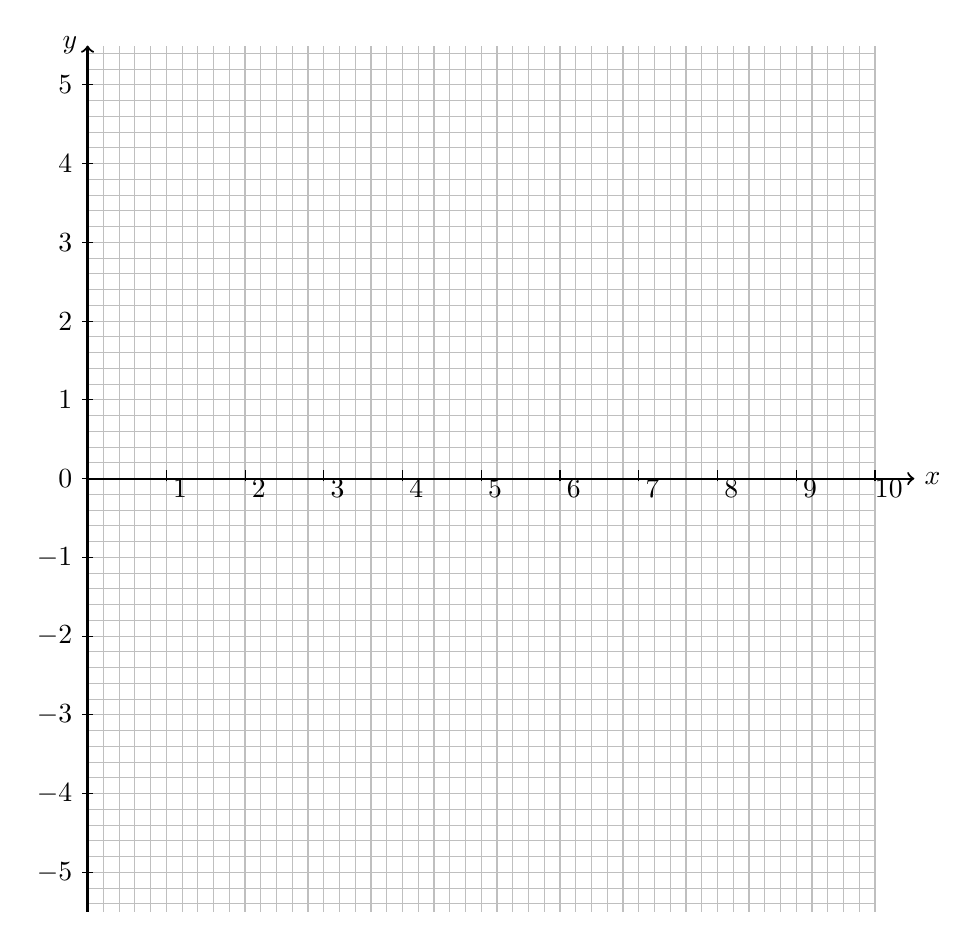
\begin{tikzpicture}

%grid
\draw [color=black,, xstep=1.0cm,ystep=1.0cm] (0,-5.5) grid (10.,5.5);
\draw [color=lightgray,, xstep=0.2cm,ystep=0.2cm] (0,-5.5) grid (10.,5.5);

\foreach \x in {,1,2,3,4,5, 6, 7, 8, 9, 10}
\draw[shift={(\x,0)},color=black] (0pt,-1pt) -- (0pt,3pt) node[below]  {$\quad \x$};

\foreach \y in {-5,-4,-3,-2,-1,0,1,2,3,4,5}
\draw[shift={(0,\y)},color=black] (2pt,0pt) -- (-2pt,0pt) node[left]  {$\y$};

\draw [thick, ->] (0,0) -- (10.5,0) node [right] {$x$};
\draw [thick, ->] (0,-5.5) -- (0,5.5) node [left] {$y$};

\end{tikzpicture}
\end{center}
\end{figure}
